% !TeX program = xelatex
\documentclass{article}
\usepackage{kotex}
\usepackage[a4paper,left=3cm, right=3cm, top=2cm, bottom=2cm]{geometry}
\usepackage{amsmath}
\usepackage{graphicx}
\usepackage{caption}
\usepackage{setspace}
\usepackage{xcolor}
\usepackage{titlesec}
\usepackage{amssymb}
\usepackage{tcolorbox}
\usepackage{amsthm}
\usepackage{multirow}
\usepackage{array}
\usepackage{booktabs}
\usepackage{tikz}
\usetikzlibrary{positioning,arrows.meta,calc}
\usepackage{pgfplots}
\pgfplotsset{compat=1.18}

\title{7.4 Optimization Using Quadratic Forms}
\date{}
\author{}
\setstretch{1.3}

\titleformat{name=\section, numberless}
  {\normalfont\large\bfseries\color{blue}}{}
  {0pt}{}
\geometry{a4paper, margin=1in}

\newcommand{\redheading}[1]{{\vspace{2mm}\noindent\Large\bfseries\color{red!55!black} #1\par}\vspace{2mm}}

\begin{document}
\maketitle

{\itshape\color{blue!45!black}
Quadratic forms arise in various problems in which the maximum or minimum value of
some quantity is required. In this section we will discuss some problems of this type.\par}

\vspace{2mm}

\redheading{Constrained Extremum Problems}

The primary goal of this section is to find the maximum and minimum values of a
quadratic form $\mathbf{x}^T A\mathbf{x}$ subject to the constraint $\|\mathbf{x}\|=1$.
Such problems arise in a wide variety of applications.

To visualize this geometrically in $R^2$: view $z=\mathbf{x}^T A\mathbf{x}$ as a surface
in $xyz$-coordinates, and $\|\mathbf{x}\|=1$ as the unit circle in the $xy$-plane. Finding
the max and min of $z$ on $\|\mathbf{x}\|=1$ amounts to finding the highest and lowest points
on the intersection of the surface with the right circular cylinder over the unit circle
(Figure 7.4.1).

\begin{figure}[ht]
\centering
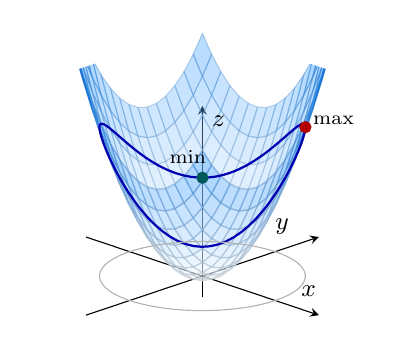
\begin{tikzpicture}
\begin{axis}[
  width=7.5cm, height=6cm,
  view={45}{30},
  xlabel={$x$}, ylabel={$y$}, zlabel={$z$},
  axis lines=center,
  ticks=none,
  zmin=-1, zmax=8,
  xmin=-1.6, xmax=1.6,
  ymin=-1.6, ymax=1.6,
  xlabel style={font=\small},
  ylabel style={font=\small},
  zlabel style={font=\small},
]
  % Surface z = 5x^2 + 5y^2 + 4xy
  \addplot3[surf, opacity=0.35, colormap/cool,
    domain=-1.2:1.2, domain y=-1.2:1.2, samples=20]
    {5*x^2 + 5*y^2 + 4*x*y};
  % Unit circle cylinder (parametric curve on surface)
  \addplot3[thick, blue!70!black, domain=0:360, samples=80, variable=\t]
    ({cos(\t)},{sin(\t)},{5*cos(\t)^2 + 5*sin(\t)^2 + 4*cos(\t)*sin(\t)});
  % Unit circle on z=0
  \addplot3[gray!60, dashed, domain=0:360, samples=60, variable=\t]
    ({cos(\t)},{sin(\t)},{0});
  % Max point
  \addplot3[mark=*, mark size=2pt, red!70!black]
    coordinates {(0.707,0.707,7)};
  \node[font=\scriptsize] at (axis cs:0.9,0.9,7.3) {max};
  % Min point
  \addplot3[mark=*, mark size=2pt, teal!70!black]
    coordinates {(-0.707,0.707,3)};
  \node[font=\scriptsize] at (axis cs:-1.1,0.9,3.3) {min};
\end{axis}
\end{tikzpicture}
\caption{The constrained max and min of $\mathbf{x}^T A\mathbf{x}$ on $\|\mathbf{x}\|=1$
are the highest and lowest points on the curve where the surface meets the unit cylinder.}
\label{fig:741}
\end{figure}

\begin{tcolorbox}[colback=red!4, colframe=red!60!black,
  title={\textbf{Theorem 7.4.1 --- Constrained Extremum Theorem}},
  boxrule=0.5mm, arc=3mm]
Let $A$ be a symmetric $n\times n$ matrix whose eigenvalues in decreasing order are
$\lambda_1\ge\lambda_2\ge\cdots\ge\lambda_n$. Then:
\begin{enumerate}
  \item[(a)] $\mathbf{x}^T A\mathbf{x}$ has a maximum value of $\lambda_1$ and a minimum
             value of $\lambda_n$, both attained on the set $\|\mathbf{x}\|=1$.
  \item[(b)] The maximum value of $\mathbf{x}^T A\mathbf{x}$ occurs at a unit eigenvector
             corresponding to $\lambda_1$.
  \item[(c)] The minimum value of $\mathbf{x}^T A\mathbf{x}$ occurs at a unit eigenvector
             corresponding to $\lambda_n$.
\end{enumerate}
\end{tcolorbox}

\textit{Proof.} By the Principal Axes Theorem (7.3.1), there is an orthogonal change of
variable $\mathbf{x}=P\mathbf{y}$ with the column vectors of $P$ ordered so that
$\lambda_1\ge\lambda_2\ge\cdots\ge\lambda_n$, giving
\begin{equation}
  \mathbf{x}^T A\mathbf{x} = \lambda_1y_1^2+\lambda_2y_2^2+\cdots+\lambda_ny_n^2 \tag{6}
\end{equation}
Since $P$ is orthogonal it is length-preserving, so $\|\mathbf{y}\|=\|\mathbf{x}\|=1$, i.e.,
\begin{equation}
  y_1^2+y_2^2+\cdots+y_n^2=1 \tag{7}
\end{equation}
From (7) and $\lambda_1\ge\cdots\ge\lambda_n$:
\[
  \lambda_n = \lambda_n(y_1^2+\cdots+y_n^2)
  \le \lambda_1y_1^2+\cdots+\lambda_ny_n^2
  \le \lambda_1(y_1^2+\cdots+y_n^2) = \lambda_1
\]
and by (6), $\lambda_n\le\mathbf{x}^T A\mathbf{x}\le\lambda_1$ for all $\|\mathbf{x}\|=1$.

If $\mathbf{x}$ is a unit eigenvector corresponding to $\lambda_1$, then
$\mathbf{x}^T A\mathbf{x}=\mathbf{x}^T(\lambda_1\mathbf{x})=\lambda_1\|\mathbf{x}\|^2=\lambda_1$,
so the maximum $\lambda_1$ is achieved. Similarly, if $\mathbf{x}$ is a unit eigenvector
corresponding to $\lambda_n$, then $\mathbf{x}^T A\mathbf{x}=\lambda_n$, so the minimum
$\lambda_n$ is achieved. $\blacksquare$

\textit{Remark.} The condition $\|\mathbf{x}\|=1$ is called a \textbf{constraint}, and the
maximum or minimum value is called a \textbf{constrained extremum}. The constraint can also
be expressed as $\mathbf{x}^T\mathbf{x}=1$ or as $x_1^2+x_2^2+\cdots+x_n^2=1$.

\subsection*{EXAMPLE 1 | Finding Constrained Extrema}

Find the maximum and minimum values of $z=5x^2+5y^2+4xy$ subject to $x^2+y^2=1$,
and the values of $x$ and $y$ at which they occur.

\textbf{SOLUTION:} In matrix notation,
\[
  z = \mathbf{x}^T A\mathbf{x} = [x\;\;y]\begin{bmatrix}5&2\\2&5\end{bmatrix}
  \begin{bmatrix}x\\y\end{bmatrix}
\]
The eigenvalues of $A$ are $\lambda_1=7$ and $\lambda_2=3$ (verify), with corresponding
unit eigenvectors
\begin{equation}
  \lambda_1=7:\;\begin{bmatrix}1/\sqrt{2}\\1/\sqrt{2}\end{bmatrix},\quad
  \lambda_2=3:\;\begin{bmatrix}-1/\sqrt{2}\\1/\sqrt{2}\end{bmatrix} \tag{1}
\end{equation}
Thus the constrained extrema are
\begin{align*}
  &\text{constrained maximum: } z=7 \text{ at } (x,y)=\bigl(\tfrac{1}{\sqrt2},\tfrac{1}{\sqrt2}\bigr)\\
  &\text{constrained minimum: } z=3 \text{ at } (x,y)=\bigl(-\tfrac{1}{\sqrt2},\tfrac{1}{\sqrt2}\bigr)
\end{align*}

\textit{Remark.} The negatives of the eigenvectors in (1) are also unit eigenvectors, so the
constrained maximum $z=7$ also occurs at $\bigl(-\tfrac{1}{\sqrt2},-\tfrac{1}{\sqrt2}\bigr)$
and the constrained minimum $z=3$ at $\bigl(\tfrac{1}{\sqrt2},-\tfrac{1}{\sqrt2}\bigr)$.

\subsection*{EXAMPLE 2 | A Constrained Extremum Problem}

A rectangle is to be inscribed in the ellipse $4x^2+9y^2=36$ with sides parallel to the
coordinate axes. Find the nonneg\-ative values of $x$ and $y$ producing the rectangle with
maximum area.

\textbf{SOLUTION:} The area of the inscribed rectangle is $z=4xy$. Rewrite the constraint
as
\[
  \Bigl(\frac{x}{3}\Bigr)^2+\Bigl(\frac{y}{2}\Bigr)^2=1
\]
and introduce new variables $x_1,y_1$ via $x=3x_1$, $y=2y_1$, so the constraint becomes
$x_1^2+y_1^2=1$ and the problem is to maximize
\[
  z = 4(3x_1)(2y_1) = 24x_1y_1
\]
Writing $z=24x_1y_1=\mathbf{x}_1^T A\mathbf{x}_1$ with
\[
  A=\begin{bmatrix}0&12\\12&0\end{bmatrix}
\]
the largest eigenvalue of $A$ is $\lambda=12$ (verify), with unit eigenvector
$\bigl[1/\sqrt{2},\;1/\sqrt{2}\bigr]^T$ (nonneg entries). The maximum area is $z=12$, occurring at
\[
  x=3x_1=\frac{3}{\sqrt{2}}, \qquad y=2y_1=\frac{2}{\sqrt{2}}
\]

\begin{figure}[ht]
\centering
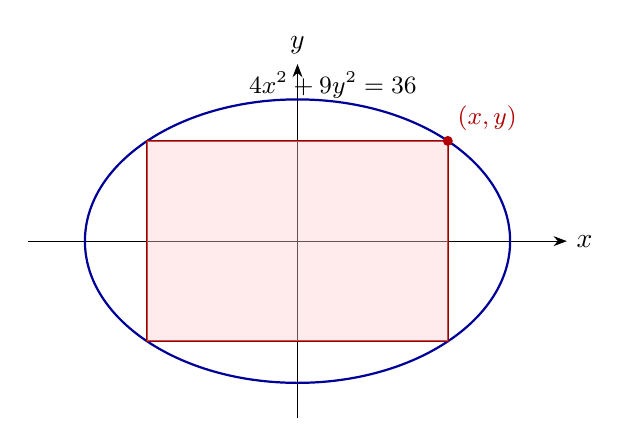
\begin{tikzpicture}[>=Stealth, scale=0.9]
  \draw[->] (-3.8,0)--(3.8,0) node[right]{$x$};
  \draw[->] (0,-2.5)--(0,2.5) node[above]{$y$};
  % Ellipse 4x^2+9y^2=36, a=3,b=2
  \draw[thick,blue!60!black] (0,0) ellipse (3 and 2);
  % Inscribed rectangle at (3/sqrt2, 2/sqrt2)
  \def\rx{2.121}\def\ry{1.414}
  \draw[thick,red!60!black]
    (-\rx,-\ry) rectangle (\rx,\ry);
  \fill[red!20,opacity=0.4]
    (-\rx,-\ry) rectangle (\rx,\ry);
  \fill[red!70!black] (\rx,\ry) circle (2pt)
    node[above right]{\small$(x,y)$};
  % Labels
  \node at (0.5,2.2) {\small$4x^2+9y^2=36$};
\end{tikzpicture}
\caption{A rectangle with maximum area inscribed in the ellipse $4x^2+9y^2=36$.}
\label{fig:742}
\end{figure}

\redheading{Constrained Extrema and Level Curves}

The \textbf{level curves} of $f(x,y)$ are the curves $f(x,y)=k$. The level curves of a
quadratic form $\mathbf{x}^T A\mathbf{x}$ on $R^2$ have equations $\mathbf{x}^T A\mathbf{x}=k$.
The maximum and minimum values of $\mathbf{x}^T A\mathbf{x}$ on $\|\mathbf{x}\|=1$ are the
largest and smallest values of $k$ for which the level curve $\mathbf{x}^T A\mathbf{x}=k$
intersects the unit circle. Typically, the extreme values correspond to level curves that
just \emph{touch} (are tangent to) the unit circle.

\subsection*{EXAMPLE 3 | Example 1 Revisited Using Level Curves}

In Example 1 the constrained maximum is $z=7$ at $\bigl(\tfrac{1}{\sqrt2},\tfrac{1}{\sqrt2}\bigr)$
and $\bigl(-\tfrac{1}{\sqrt2},-\tfrac{1}{\sqrt2}\bigr)$, and the constrained minimum is $z=3$
at $\bigl(-\tfrac{1}{\sqrt2},\tfrac{1}{\sqrt2}\bigr)$ and $\bigl(\tfrac{1}{\sqrt2},-\tfrac{1}{\sqrt2}\bigr)$.
Geometrically, the level curve $5x^2+5y^2+4xy=7$ just touches the unit circle at the two
maximum points (3), and the level curve $5x^2+5y^2+4xy=3$ just touches the unit circle at
the two minimum points (4) --- see Figure 7.4.5.

\begin{figure}[ht]
\centering
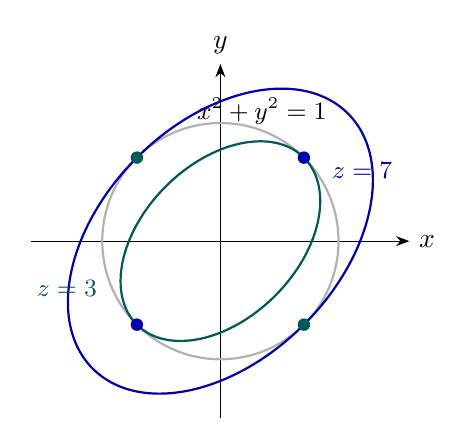
\begin{tikzpicture}[>=Stealth, scale=1.5]
  \draw[->] (-1.6,0)--(1.6,0) node[right]{$x$};
  \draw[->] (0,-1.5)--(0,1.5) node[above]{$y$};
  % Unit circle
  \draw[thick,gray!60] (0,0) circle (1);
  \node at (0.35,1.1) {\small$x^2+y^2=1$};
  % Level curve z=7: 5x^2+4xy+5y^2=7
  % This is an ellipse; rotation angle theta=pi/4 diagonalizes it
  % In rotated frame: 7x'^2 + 3y'^2 = 7, i.e. x'^2 + y'^2/7*3 = 1
  % semi-axes: a=1 (x'), b=sqrt(7/3) (y')
  % Rotated by -45 deg
  \begin{scope}[rotate=-45]
    \draw[thick,blue!70!black] (0,0) ellipse (1 and {sqrt(7/3)});
  \end{scope}
  \node[blue!70!black] at (1.2,0.6) {\small$z=7$};
  % Level curve z=3: 5x^2+4xy+5y^2=3
  % In rotated frame: 7x'^2 + 3y'^2 = 3, i.e. x'^2/(3/7) + y'^2 = 1
  % semi-axes: a=sqrt(3/7) (x'), b=1 (y')
  \begin{scope}[rotate=-45]
    \draw[thick,teal!70!black] (0,0) ellipse ({sqrt(3/7)} and 1);
  \end{scope}
  \node[teal!70!black] at (-1.3,-0.4) {\small$z=3$};
  % Tangent points
  \foreach \pt in {(0.707,0.707),(-0.707,-0.707)}{
    \fill[blue!70!black] \pt circle (1.5pt);
  }
  \foreach \pt in {(-0.707,0.707),(0.707,-0.707)}{
    \fill[teal!70!black] \pt circle (1.5pt);
  }
\end{tikzpicture}
\caption{Level curves of $z=5x^2+5y^2+4xy$ tangent to the unit circle at the constrained
extrema.}
\label{fig:745}
\end{figure}

\redheading{Relative Extrema of Functions of Two Variables}
\textit{(Calculus Required)}

We now show how quadratic forms can be used to study characteristics of real-valued
functions of two variables.

Recall that if $f(x,y)$ has first-order partial derivatives, its relative maxima and minima
occur at \textbf{critical points} where
\[
  f_x(x,y)=0 \quad\text{and}\quad f_y(x,y)=0
\]
The behavior of $f$ at a critical point $(x_0,y_0)$ is determined by the sign of
\begin{equation}
  D(x,y)=f(x,y)-f(x_0,y_0) \tag{5}
\end{equation}
at nearby points $(x,y)\neq(x_0,y_0)$:
\begin{itemize}
  \item $D>0$ near $(x_0,y_0)$: $f$ has a \textbf{relative minimum} at $(x_0,y_0)$
  \item $D<0$ near $(x_0,y_0)$: $f$ has a \textbf{relative maximum} at $(x_0,y_0)$
  \item $D$ takes both signs: $f$ has a \textbf{saddle point} at $(x_0,y_0)$
\end{itemize}

The following theorem, proved in calculus, makes it possible to analyze critical points
using second-order partial derivatives.

\begin{tcolorbox}[colback=red!4, colframe=red!60!black,
  title={\textbf{Theorem 7.4.2 --- Second Derivative Test}}, boxrule=0.5mm, arc=3mm]
Suppose $(x_0,y_0)$ is a critical point of $f(x,y)$ and $f$ has continuous second-order
partial derivatives in some circular region centered at $(x_0,y_0)$. Then:
\begin{enumerate}
  \item[(a)] $f$ has a relative minimum at $(x_0,y_0)$ if
    \[f_{xx}(x_0,y_0)f_{yy}(x_0,y_0)-f_{xy}^2(x_0,y_0)>0 \;\text{ and }\; f_{xx}(x_0,y_0)>0\]
  \item[(b)] $f$ has a relative maximum at $(x_0,y_0)$ if
    \[f_{xx}(x_0,y_0)f_{yy}(x_0,y_0)-f_{xy}^2(x_0,y_0)>0 \;\text{ and }\; f_{xx}(x_0,y_0)<0\]
  \item[(c)] $f$ has a saddle point at $(x_0,y_0)$ if
    \[f_{xx}(x_0,y_0)f_{yy}(x_0,y_0)-f_{xy}^2(x_0,y_0)<0\]
  \item[(d)] The test is inconclusive if $f_{xx}(x_0,y_0)f_{yy}(x_0,y_0)-f_{xy}^2(x_0,y_0)=0$.
\end{enumerate}
\end{tcolorbox}

The expression $f_{xx}f_{yy}-f_{xy}^2$ can be expressed using the \textbf{Hessian matrix}
(named for the German mathematician Ludwig Otto Hesse, 1811--1874):
\[
  H(x,y) = \begin{bmatrix}f_{xx}(x,y)&f_{xy}(x,y)\\f_{xy}(x,y)&f_{yy}(x,y)\end{bmatrix}
\]
Then
\[
  \det[H(x_0,y_0)] = \begin{vmatrix}f_{xx}(x_0,y_0)&f_{xy}(x_0,y_0)\\f_{xy}(x_0,y_0)&f_{yy}(x_0,y_0)\end{vmatrix}
  = f_{xx}f_{yy}-f_{xy}^2\big|_{(x_0,y_0)}
\]
Theorem 7.4.2 can now be reformulated in terms of the definiteness of $H(x_0,y_0)$.

\begin{tcolorbox}[colback=red!4, colframe=red!60!black,
  title={\textbf{Theorem 7.4.3 --- Hessian Form of the Second Derivative Test}},
  boxrule=0.5mm, arc=3mm]
Suppose $(x_0,y_0)$ is a critical point of $f(x,y)$ and $f$ has continuous second-order
partial derivatives in some circular region centered at $(x_0,y_0)$. If $H(x_0,y_0)$ is
the Hessian of $f$ at $(x_0,y_0)$, then:
\begin{enumerate}
  \item[(a)] $f$ has a relative minimum at $(x_0,y_0)$ if $H(x_0,y_0)$ is positive definite.
  \item[(b)] $f$ has a relative maximum at $(x_0,y_0)$ if $H(x_0,y_0)$ is negative definite.
  \item[(c)] $f$ has a saddle point at $(x_0,y_0)$ if $H(x_0,y_0)$ is indefinite.
  \item[(d)] The test is inconclusive otherwise.
\end{enumerate}
\end{tcolorbox}

\textit{Proof of (a).} If $H(x_0,y_0)$ is positive definite, then Theorem 7.3.4 implies
all principal submatrix determinants are positive. In particular,
\[
  \det[H(x_0,y_0)] = f_{xx}(x_0,y_0)f_{yy}(x_0,y_0)-f_{xy}^2(x_0,y_0)>0
\]
and $\det[f_{xx}(x_0,y_0)]=f_{xx}(x_0,y_0)>0$, so $f$ has a relative minimum at $(x_0,y_0)$
by Theorem 7.4.2(a). $\blacksquare$

\textit{(The proofs of parts (b)--(d) are analogous and are left as exercises.)}

\subsection*{EXAMPLE 4 | Using the Hessian to Classify Relative Extrema}

Find the critical points of $f(x,y)=\tfrac{1}{3}x^3+xy^2-8xy+3$ and use the eigenvalues
of the Hessian matrix at those points to classify each as a relative maximum, relative
minimum, or saddle point.

\textbf{SOLUTION:} The first and second partial derivatives are
\[
  f_x = x^2+y^2-8y,\quad f_y = 2xy-8x = 2x(y-4),\quad
  f_{xx}=2x,\quad f_{yy}=2x,\quad f_{xy}=2y-8
\]
Setting $f_y=0$: either $x=0$ or $y=4$.
\begin{itemize}
  \item $x=0$: $f_x=y^2-8y=y(y-8)=0$ gives $y=0$ or $y=8$.
  \item $y=4$: $f_x=x^2+16-32=x^2-16=0$ gives $x=\pm4$.
\end{itemize}
The four critical points are $(0,0)$, $(0,8)$, $(4,4)$, $(-4,4)$. The Hessian matrix is
\[
  H(x,y) = \begin{bmatrix}2x&2y-8\\2y-8&2x\end{bmatrix}
\]
Evaluating at the critical points:
\[
  H(0,0) = \begin{bmatrix}0&-8\\-8&0\end{bmatrix},\quad
  H(0,8) = \begin{bmatrix}0&8\\8&0\end{bmatrix},\quad
  H(4,4) = \begin{bmatrix}8&0\\0&8\end{bmatrix},\quad
  H(-4,4) = \begin{bmatrix}-8&0\\0&-8\end{bmatrix}
\]

\begin{center}
\renewcommand{\arraystretch}{1.3}
\begin{tabular}{|c|c|c|c|}
\hline
\textbf{Critical Point $(x_0,y_0)$} & $\lambda_1$ & $\lambda_2$ & \textbf{Classification}\\
\hline
$(0,0)$ & $8$ & $-8$ & Saddle point\\
\hline
$(0,8)$ & $8$ & $-8$ & Saddle point\\
\hline
$(4,4)$ & $8$ & $8$ & Relative minimum\\
\hline
$(-4,4)$ & $-8$ & $-8$ & Relative maximum\\
\hline
\end{tabular}
\end{center}

\vspace{3mm}
\noindent\rule{\linewidth}{0.5pt}

\section*{Exercise Set 7.4}

\noindent\textit{In Exercises 1--4, find the maximum and minimum values of the quadratic
form subject to the constraint $x^2+y^2=1$, and determine the values of $x$ and $y$ at
which the maximum and minimum occur.}

\begin{enumerate}

\item $5x^2-y^2$

\item[2.] $xy$

\item[3.] $3x^2+7y^2$

\noindent\textit{In Exercises 5--6, find the maximum and minimum values of the quadratic
form subject to the constraint $x^2+y^2+z^2=1$, and determine the values of $x$, $y$, $z$
at which the maximum and minimum occur.}

\item[5.] $9x^2+4y^2+3z^2$

\noindent\textit{In Exercises 7--8, use the method of Example 2 to find the maximum and
minimum values of the given quadratic form subject to the stated constraint.}

\item[7.] $xy$; \; $4x^2+8y^2=16$

\item[8.] $x^2+xy+2y^2$; \; $x^2+3y^2=16$

\noindent\textit{In Exercises 9--10, draw the unit circle and the level curves of the
quadratic form corresponding to the constrained maximum and minimum. Show that the unit
circle intersects each of these curves in exactly two places, label those intersection
points, and verify that the constrained extrema occur at those points.}

\item[10.] $xy$

\noindent\textit{In Exercises 11--12, (a) show that the given function has critical points
at the stated locations, and (b) use the Hessian form of the second derivative test to
show the stated classification.}

\item[11.] $f(x,y)=4xy-x^4-y^4$

\textbf{a.}\ Critical points at $(0,0)$, $(1,1)$, and $(-1,-1)$.

\textbf{b.}\ $f$ has relative maxima at $(1,1)$ and $(-1,-1)$, and a saddle point at $(0,0)$.

\item[12.] $f(x,y)=x^3-6xy-y^3$

\textbf{a.}\ Critical points at $(0,0)$ and $(-2,2)$.

\textbf{b.}\ $f$ has a relative maximum at $(-2,2)$ and a saddle point at $(0,0)$.

\noindent\textit{In Exercises 13--16, find the critical points of $f$, if any, and classify
them as relative maxima, relative minima, or saddle points.}

\item[13.] $f(x,y) = x^3-3xy-y^3$

\item[15.] $f(x,y) = x^2+2y^2-x^2y$

\item[16.] $f(x,y) = x^3+y^3-3x-3y$

\item[17.] A rectangle whose center is at the origin and whose sides are parallel to the
coordinate axes is to be inscribed in the ellipse $x^2+25y^2=25$. Use the method of
Example 2 to find nonneg\-ative values of $x$ and $y$ that produce the inscribed rectangle
with maximum area.

\item[18.] Suppose $\mathbf{x}$ is a unit eigenvector of a matrix $A$ corresponding to an
eigenvalue $\lambda=2$. What is the value of $\mathbf{x}^T A\mathbf{x}$?

\noindent\textit{\textbf{Working with Proofs}}

\item[21.] Suppose $A$ is an $n\times n$ symmetric matrix and $q(\mathbf{x})=\mathbf{x}^T A\mathbf{x}$,
where $\mathbf{x}$ is a vector in $R^n$ expressed in column form. What can you say about
the value of $q$ if $\mathbf{x}$ is a unit eigenvector corresponding to an eigenvalue
$\lambda$ of $A$?

\item[22.] Prove: If $\mathbf{x}^T A\mathbf{x}$ is a quadratic form whose minimum and maximum
values subject to the constraint $\|\mathbf{x}\|=1$ are $m$ and $M$, respectively, then for
each number $c$ in the interval $m\le c\le M$ there is a unit vector $\mathbf{x}_c$ such
that $\mathbf{x}_c^T A\mathbf{x}_c=c$.

[$Hint$: In the case $m<M$, let $\mathbf{u}_m$ and $\mathbf{u}_M$ be unit eigenvectors of
$A$ such that $\mathbf{u}_m^T A\mathbf{u}_m=m$ and $\mathbf{u}_M^T A\mathbf{u}_M=M$, and let
\[
  \mathbf{x}_c = \sqrt{\frac{M-c}{M-m}}\,\mathbf{u}_m + \sqrt{\frac{c-m}{M-m}}\,\mathbf{u}_M
\]
Show that $\mathbf{x}_c^T A\mathbf{x}_c=c$.]

\end{enumerate}

\end{document}
